\chapter{Objekty v~prostoru}

Souřadné systémy nám umožňují popisovat objekty v~prostoru. Nyní si ukážeme, jak je to možné. 

\section{Bod}

Začněme nejjednodušším objektem, kterým je bod. Bod v~\(n\)-rozměrném prostoru, označme jej \(P\), lze popsat \(n\) souřadnicemi \([P_1, P_2, ..., P_n]\). Souřadnice nemají žádný parametr, jsou konstantní. Říkáme, že bod je bezrozměrný.

\section{Oblast}

Mějme metrický prostor \((M, d)\) a~množinu bodů \(\Omega \subset M\). Pak můžeme zavést následující klasifikaci bodů.

Bod nazýváme vnitřním bodem pokud existuje jeho \(\delta\)-okolí takové, že všechny body v~něm obsažené leží v~množině \(\Omega\):

\begin{equation}
\exists \delta > 0 \ \mathrm{U}_{\delta}(P) \subset \Omega
\end{equation}

Bod nazýváme hraničním bodem pokud každé jeho \(\delta\)-okolí obsahuje alespoň jeden bod ležící v~množině \(\Omega\) a~alespoň jeden bod neležící v~množině \(\Omega\):

\begin{equation}
\forall \delta > 0 \ \mathrm{U}_{\delta}(P) \cap \Omega \neq \emptyset \land \mathrm{U}_{\delta}(P) \cap (M \setminus \Omega) \neq \emptyset
\end{equation}

Množinu všech hraničních bodů nazýváme hranicí množiny \(\Omega\) a~značíme ji \(\partial \Omega\).

Vnitřní bod je vždy obsažen v~množině. Hraniční bod může ale nemusí být obsažen v~množině. Hraniční bod nemůže být vnitřní.

Pokud jsou všechny body množiny vnitřní, tedy pokud množina neobsahuje svoji hranici, pak ji nazýváme otevřenou. Pokud každé dva body množiny \(\Omega\) lze spojit křivkou složenou z~konečného množství úseček (tedy lomenou čarou), která celá leží v~množině \(\Omega\), pak množinu \(\Omega\) nazýváme souvislou.  

\begin{fact}
Otevřenou souvislou množinu nazýváme oblastí.
\end{fact}

\begin{fact}
Sjednocením oblasti \(\Omega\) s~její hranicí označujeme \(\overline{\Omega} = \Omega \cup \partial \Omega\). Získáme tak uzavřenou oblast. 
\end{fact}

Na obrázku~\ref{img:oblast} je příklad oblasti. Na obrázku jsou zobrazeny 3 body včetně jejich \(\delta\)-okolí. Bod~\(A\) je vnitřním bodem, bod \(B\) je hraničním bodem a~neleží tedy v~oblasti stejně jako bod \(C\). Na obrázku~\ref{img:uzavrena_oblast} je nakreslena uzavřená oblast. Je-li hranice obsažena v~množině, pak ji kreslíme plnou čarou, není-li obsažena v~množině, tak ji kreslíme přerušovanou čarou.

\begin{figure}
\begin{center}
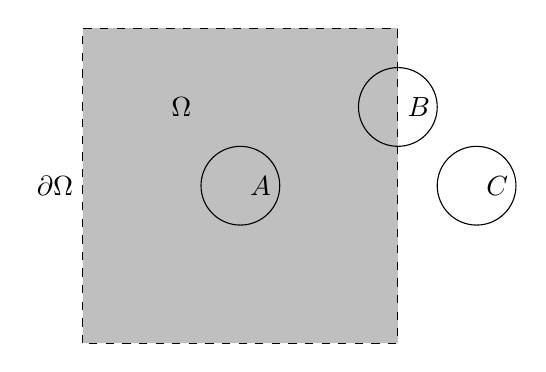
\begin{tikzpicture}

\draw[dashed,fill=lightgray] (-2, -2) -- (-2, 2) -- (2, 2) -- (2, -2) -- (-2, -2);

\draw (-1, 1) node[anchor=west]{\(\Omega\)};
\draw (-2, 0) node[anchor=east]{\(\partial \Omega\)};

\drawcross{0}{0}{0.1};
\draw (0, 0) circle[radius=0.5];
\draw (0, 0) node[anchor=west]{\(A\)};

\drawcross{2}{1}{0.1};
\draw (2, 1) circle[radius=0.5];
\draw (2, 1) node[anchor=west]{\(B\)};

\drawcross{3}{0}{0.1};
\draw (3, 0) circle[radius=0.5];
\draw (3, 0) node[anchor=west]{\(C\)};

\end{tikzpicture}
\caption{Oblast}
\end{center}
\label{img:oblast}
\end{figure}

\begin{figure}
\begin{center}
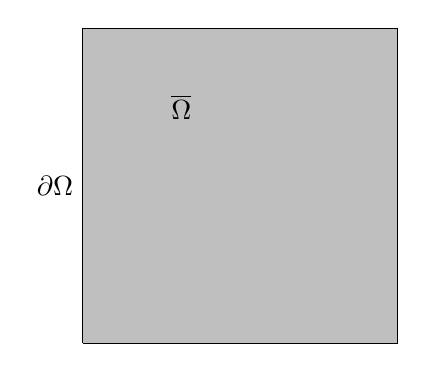
\begin{tikzpicture}

\draw[fill=lightgray] (-2, -2) -- (-2, 2) -- (2, 2) -- (2, -2) -- (-2, -2);

\draw (-1, 1) node[anchor=west]{\(\overline{\Omega}\)};
\draw (-2, 0) node[anchor=east]{\(\partial \Omega\)};

\end{tikzpicture}
\caption{Uzavřená oblast}
\end{center}
\label{img:uzavrena_oblast}
\end{figure}

\section{Křivka}

Křivku v~\(n\)-rozměrném prostoru, označme ji \(\Gamma\), lze popsat sadou \(n\) funkcí souřadnic \([\Gamma_1(t), \Gamma_2(t), ..., \Gamma_n(t)]\). Funkce souřadnic mají jeden parametr \(t\), říkáme, že křivka je jednorozměrná. Někdy pro zjednodušení místo o~sadě funkcí hovoříme o~funkci jedné.

Parametr \(t\) probíhá po zvoleném intervalu \(I\), který je sjednocením nejvýše \(m\) disjuktních otevřených intervalů \(I_i\) spolu s~jejich hranicemi. Tedy 

\begin{equation}
I = \bigcup_{i=1}^m \overline{I_i} 
\end{equation}

Otevřený interval je oblastí, proto \(\overline{I_i}\) je uzavřený interval. Dále musí pro \(i \neq j\) platit: 

\begin{equation}
I_i \cap I_j = \emptyset
\end{equation}

Zaveďme označení:

\begin{equation}
\vect{\Gamma} = [\Gamma_1(t), \Gamma_2(t), ..., \Gamma_n(t)]
\end{equation}

a

\begin{equation}
\frac{\partial \vect{\Gamma}}{\partial t} = \left(\frac{\partial \Gamma_1}{\partial t}, \frac{\partial \Gamma_2}{\partial t}, ..., \frac{\partial \Gamma_n}{\partial t} \right)
\end{equation}

Pak předpokládáme:

\begin{itemize}

\item funkce \(\Gamma_i(t)\) jsou spojité, tedy:
\begin{equation}
\forall t_0 \in I \setminus \partial I: \lim_{t \to t_0} \vect{\Gamma}(t) = \vect{\Gamma}(t_0)
\end{equation}

\item derivace \(\frac{\partial \Gamma_i}{\partial t}\) jsou na intervalech \(I_j\) spojité, tedy:
\begin{equation}
\forall j \in 1...m \ \forall t_0 \in I_j \ \lim_{t \to t_0} \frac{\partial \vect{\Gamma}}{\partial t}(t) = \frac{\partial \vect{\Gamma}}{\partial t}(t_0)
\end{equation}
Na celém intervalu \(I\) jsou tedy derivace po částech spojité.

\item derivace \(\frac{\partial \Gamma_i}{\partial t}\) nejsou na intervalech \(I_j\) v~určitém bodě všechny nulové, tedy:
\begin{equation}
\forall j \in 1...m \ \forall t_0 \in I_j \ \frac{\partial \vect{\Gamma}}{\partial t}(t_0) \neq \vect{0}
\end{equation}
Na celém intervalu \(I\) tedy mohou být všechny derivace nulové jen v~konečném počtu bodů.

\end{itemize}

První předpoklad zajišťuje, že je křivka spojitá - že je v~celku. Druhý předpoklad zajišťuje, že až na konečný počet bodů je křivka hladká. Křivka se tak skládá z~konečného počtu hladkých úseků na intervalech \(I_i\), které jsou vzájemně spojené a~ve spojích se může křivka "zlomit". Tímto předpokladem tedy vylučujeme například fraktální křivky, pro technickou praxi je však tato definice křivek dostatečná. Třetí předpoklad říká, že křivka nemůže v~určitém podintervalu \(I\) uváznout na místě. 

Pokud \(I = <t_1, t_2>\), pak mohou nastat dva případy. Buď \(\vect{\Gamma}(t_1) = \vect{\Gamma}(t_2)\), pak křivku \(\Gamma\) nazýváme uzavřenou. Takováto křivka nemá hranici. V~opačném případě jsou hranicemi křivky body \(\vect{\Gamma}(t_1)\) a~ \(\vect{\Gamma}(t_2)\).

Křivku je možné v~okolí bodu \(t_0\) linearizovat - nahradit přímkou. Rovnice takovéto přímky je:

\begin{equation}
P = \vect{\Gamma}(t_0) + (t - t_0) \cdot \frac{\partial \vect{\Gamma}}{\partial t}(t_0)
\end{equation}

Výraz 

\begin{equation}
\mathrm{d}\vect{l} = \frac{\partial \vect{\Gamma}}{\partial t} \cdot \mathrm{d}t 
\end{equation}

představuje element křivky. Vektor \(\mathrm{d}\vect{l}\) má v~každém bodě křivky směr její tečny a~velikost posunutí po křivce odpovídající změně parametru \(t\) o~\(\mathrm{d}t\).

\section{Plocha}

Plochu v~\(n\)-rozměrném prostoru, označme ji \(S\), lze popsat sadou \(n\) funkcí souřadnic \([S_1(t, u), S_2(t, u), ..., S_n(t, u)]\). Funkce souřadnic mají dva parametry \(t\) a~\(u\), říkáme, že plocha je dvojrozměrná.

Zaveďme označení:

\begin{equation}
\vect{S} = [S_1(t, u), S_2(t, u), ..., S_n(t, u)]
\end{equation}

a

\begin{equation}
\frac{\partial \vect{S}}{\partial t} = \left(\frac{\partial S_1}{\partial t}, \frac{\partial S_2}{\partial t}, ..., \frac{\partial S_n}{\partial t} \right)
\end{equation}

\begin{equation}
\frac{\partial \vect{S}}{\partial u} = \left(\frac{\partial S_1}{\partial u}, \frac{\partial S_2}{\partial u}, ..., \frac{\partial S_n}{\partial u} \right)
\end{equation}

Parametry \(t\) a~\(u\) probíhají po určité oblasti \(\Omega\), která je sjednocením \(m\) oblastí \(\Omega_i\) spolu s~jejich hranicemi:

\begin{equation}
\Omega = \bigcup_{i=1}^m \overline{\Omega_i}
\end{equation}

\begin{equation}
i \neq j \rightarrow \Omega_i \cap \Omega_j = \emptyset
\end{equation}

Pak předpokládáme:

\begin{itemize}
\item funkce \(S_i(t, u)\) jsou spojité, tedy \(\forall [t_0, u_0] \in \Omega \setminus \partial \Omega: \lim_{[t, u] \to [t_0, u_0]} \vect{S}(t, u) = \vect{S}(t_0, u_0)\)

\item derivace \(\frac{\partial S_i}{\partial t}\) a~\(\frac{\partial S_i}{\partial u}\) jsou v~oblastech \(\Omega_j\) spojité, tedy:
\begin{equation}
\forall j \in 1...m \ \forall [t_0, u_0] \in \Omega_j \ \lim_{[t, u] \to [t_0, u_0]} \frac{\partial \vect{S}}{\partial t}(t, u) = \frac{\partial \vect{S}}{\partial t}(t_0, u_0)
\end{equation}

\item derivace \(\frac{\partial \vect{S}}{\partial t}\) a~\(\frac{\partial \vect{S}}{\partial u}\) nejsou na oblastech \(\Omega_j\) v~určitém bodě kolineární, tedy:
\begin{equation}
\forall j \in 1...m \ \forall [t_0, u_0] \in \Omega_j \not \exists [k_1, k_2] \neq [0, 0] \ k_1 \cdot \frac{\partial \vect{S}}{\partial t}(t_0, u_0) + k_2 \cdot \frac{\partial \vect{S}}{\partial u}(t_0, u_0) = \vect{0}
\end{equation}

\item hranici plochy \(\partial \Omega\), pokud existuje, tvoří křivky.

\end{itemize}

Ve třírozměrném prostoru výraz 

Povšimněme si, že vektory \(\frac{\partial \vect{S}}{\partial t}\) a \(\frac{\partial \vect{S}}{\partial u}\) jsou (v daném bodě) tečné k ploše \(S\). Proto ve třírozměrném prostoru vektorový součin \(\frac{\partial S}{\partial t} \times \frac{\partial S}{\partial u}\) má směr normály. Ne však nutně shodnou orientaci. Proto výraz

\begin{equation}
\label{eq:element_plochy}
\mathrm{d} \vect{s} = \frac{\partial \vect{S}}{\partial t} \times \frac{\partial \vect{S}}{\partial u} \mathrm{d}t \ \mathrm{d}u
\end{equation}

představuje element plochy, který má v~každém bodě plochy směr její normály (až na orientaci) a~velikost odpovídající ploše, kterou vyvolá změna parametrů o~\(\mathrm{d}t\) a~\(\mathrm{d}u\).

\section{Definice pomocí hranice}

Křivku a~plochu jsme definovali pomocí jejich parametrických rovnic. Mohli bychom pokračovat dále a~definovat těleso pomocí parametrické rovnice. V~praxi to ale není nutné, protože většinou nepotřebujeme vícerozměrný prostor než trojrozměrný.

Ve dvojrozměrném prostoru uzavřená neprotínající-se křivka rozděluje prostor na dvě plochy a~tvoří jejich hranici. Pokud tedy identifikujeme jednu z~nich, tak její hranice plně určuje tuto plochu. 

Obdobně ve trojrozměrném prostoru uzavřená neprotínající-se plocha rozděluje prostor na dvě tělesa a~tvoří jejich hranici. Pokud tedy identifikujeme jedno z~nich, tak její hranice plně určuje toto těleso.
